\documentclass[10pt,twocolumn,letterpaper]{article}

\usepackage{cvpr}
\usepackage{times}
\usepackage{epsfig}
\usepackage{graphicx}
\usepackage{amsmath}
\usepackage{amssymb}

% Include other packages here, before hyperref.

% If you comment hyperref and then uncomment it, you should delete
% egpaper.aux before re-running latex.  (Or just hit 'q' on the first latex
% run, let it finish, and you should be clear).
\usepackage[breaklinks=true,bookmarks=false]{hyperref}

\cvprfinalcopy % *** Uncomment this line for the final submission

\def\cvprPaperID{****} % *** Enter the CVPR Paper ID here
\def\httilde{\mbox{\tt\raisebox{-.5ex}{\symbol{126}}}}

% Pages are numbered in submission mode, and unnumbered in camera-ready
%\ifcvprfinal\pagestyle{empty}\fi
% \setcounter{page}{4321}
\begin{document}
\title{CSE473 Final Project: Vision-based Micromouse Maze Wall Detection}

\author{Scott Will, Mack Ward\\
University at Buffalo\\
Amherst, NY 14261\\
{\tt\small scottwil@buffalo.edu, mward4@buffalo.edu}
}

\maketitle
%\thispagestyle{empty}

%%%%%%%%% ABSTRACT
\begin{abstract}
	Since the late 1970s, students and professional engineers alike have competed in Micromouse, an event in which teams
	of participants construct wheeled robots that attempt to autonomously traverse and solve planar mazes in as little
	time as possible.  A common solution strategies adopted by competitors is a two-stage process: first, a mouse
	explores the maze and incrementally generates a virtual representation of the maze layout in its internal memory,
	then computes the optimal path from the starting position to the center of the maze, and finally returns to the
	starting position and moves along the optimal path.  Although this approach is effective and reliable, most of the
	total time spent in transit by the mouse tends to be devoted to the exploration phase.  To reduce this time, we
	propose a much different strategy: using a camera mounted on the mouse at sufficient height and techniques from
	computer vision and image processing, generate an image of the maze from the perspective of a viewer looking down
	from above, extract the locations of the maze walls programmatically, and proceed to solve the maze by directly
	moving to its center.
\end{abstract}

%%%%%%%%% BODY TEXT
\section{Introduction}
\label{sec:introduction}
%-------------------------------------------------------------------------

\subsection{Competition rules}
\label{sub:rules}
In order to lessen the burden of constructing appropriately-sized vehicles, typical Micromouse events follow standard
rules and maze-guidelines.  We reproduce them here for thoroughness (adapted from the official rules from the IEEE
Region 1 Micromouse
Competition) []:

\subsubsection{Rules for the micromouse}
\label{ssub:mouserules}
\begin{enumerate}
	\item A Micromouse shall be self-contained (no remote controls). A Micromouse shall not use an energy source
	employing a combustion process.
	\item A Micromouse shall not leave any part of its body behind while negotiating the maze.
	\item A Micromouse shall not jump over, fly over, climb, scratch, cut, burn, mark, damage, or destroy
	the walls of the maze.
	\item A Micromouse shall not be larger either in length or in width, than 25 centimeters. The dimensions of a
	Micromouse that changes its geometry during a run shall not be greater than $25\ \textrm{cm} \times 25\
	\textrm{cm}$. There are no restrictions on the height of a Micromouse.
\end{enumerate}

\begin{figure}[b]
\begin{center}
	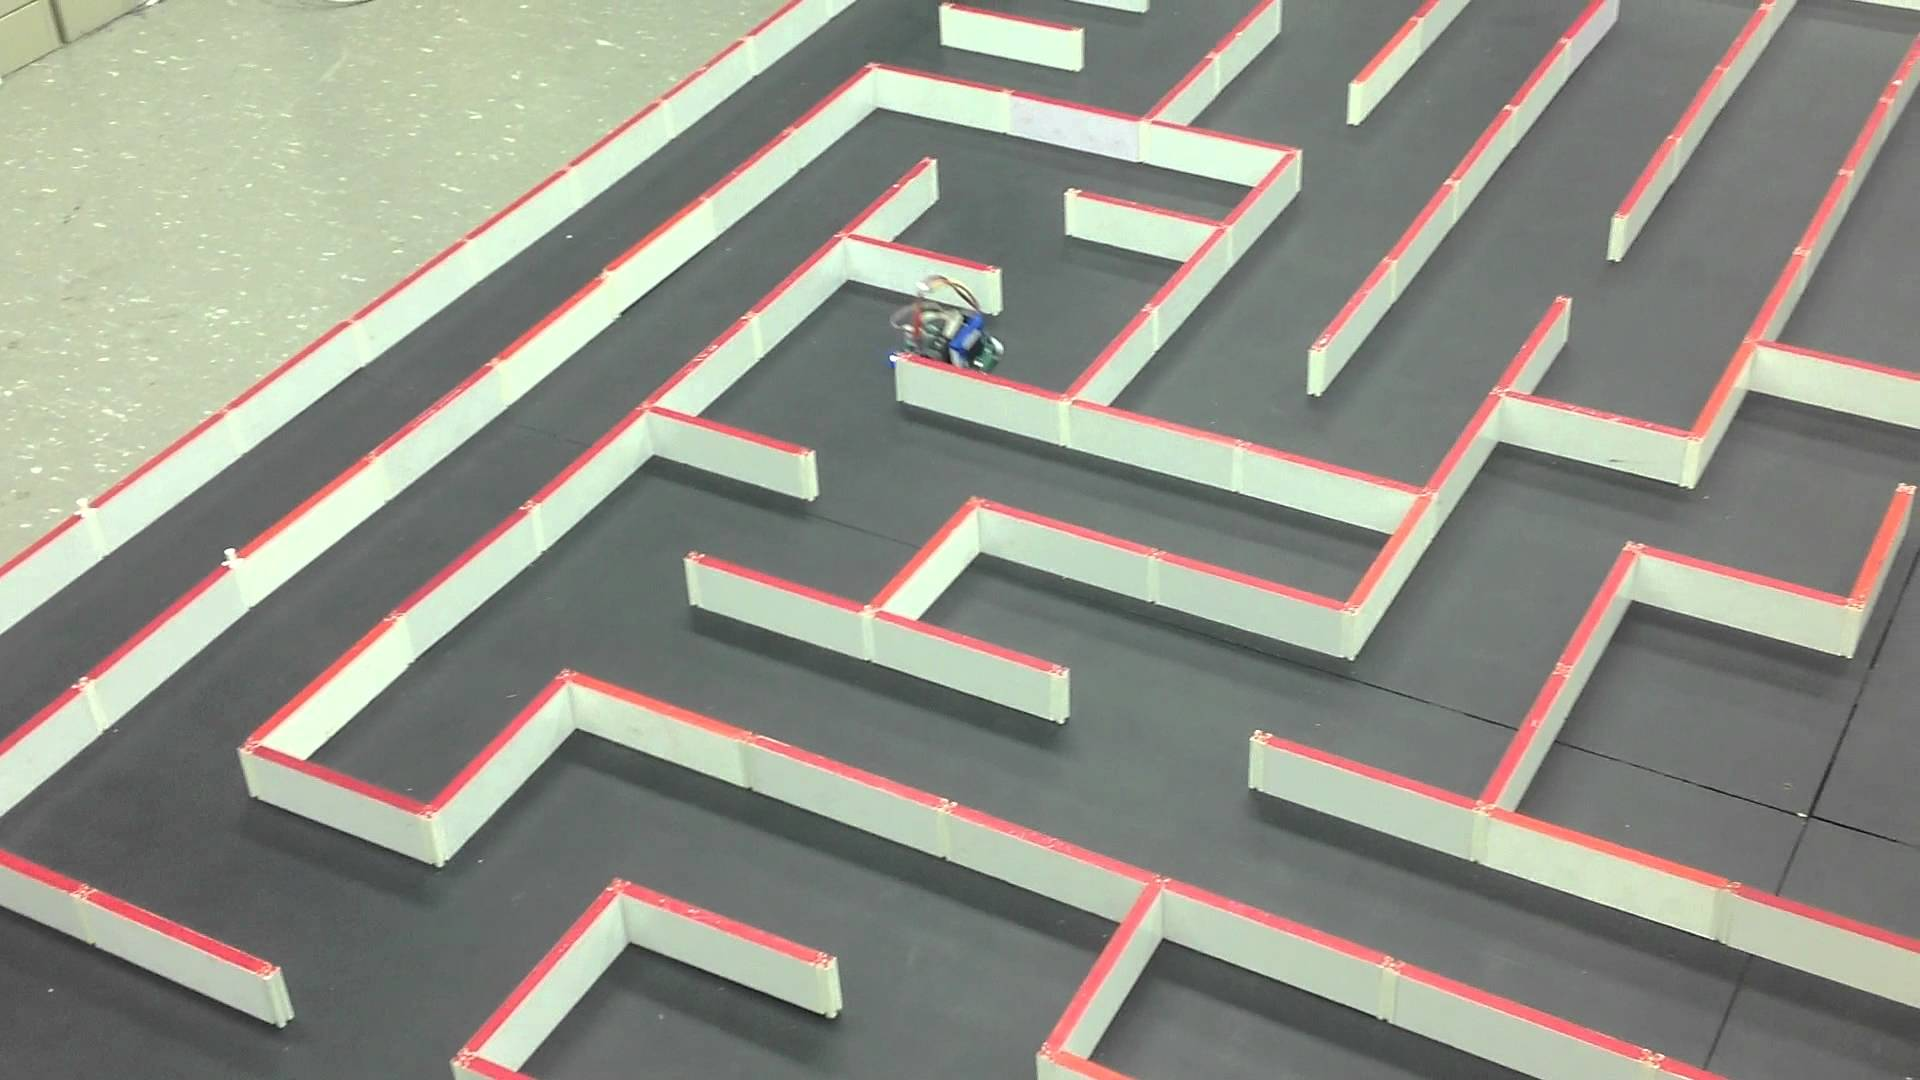
\includegraphics[width=0.8\linewidth]{maze_and_mouse.jpg}
\end{center}
\caption{A typical Micromouse and maze}
\label{fig:mouse_and_maze}
\end{figure}


\subsubsection{Rules for the maze}
\label{ssub:mazerules}
\begin{enumerate}
	\item The maze is composed of multiples of an $18\ \textrm{cm} \times 18\ \textrm{cm}$ unit square. The maze
       comprises $16 \times 16$ unit squares. The walls of the maze are $5\ \textrm{cm}$ high and $1.2\ \textrm{cm}$
       thick (assume 5\% tolerance for mazes). The outside wall encloses the entire maze.
	\item The sides of the maze walls are white, the tops of the walls are red, and the floor is black. The maze is made
       of wood, finished with non-gloss paint.
	\item The start of the maze is located at one of the four corners. The start square is bounded on three sides by
       walls. The start line is located between the first and second squares. That is, as the mouse exits the corner
       square, the time starts. The destination goal is the four cells at the center of the maze. At the center of this
       zone is a post, $20\ \textrm{cm}$ high and each side $2.5\ \textrm{cm}$. (This post may be removed if requested.)
       The destination square has only one entrance.
	\item Small square zones (posts), each $1.2\ \textrm{cm} \times 1.2\ \textrm{cm}$, at the four corners of each unit
       square are called lattice points. The maze is so constituted that there is at least one wall at each lattice
       point.
	\item Multiple paths to the destination square are allowed and are to be expected. The destination square will be
       positioned so that a wall-hugging mouse will NOT be able to find it.
\end{enumerate}

\subsection{Common Solution Methods}
\label{sub:solutionmethods}
As briefly described above, a great majority of teams tend to follow roughly the same high-level steps for producing a
mouse capable of reaching the center of a maze meeting the above specifications:

\begin{enumerate}
	\item Fully traverse the maze (including all dead-end routes) and generate an internal representation of the maze
	topology
	\item Use one or more searching algorithms such as bread-first or depth-first search, to find the optimal path from
	the starting point to the maze center
	\item Move along the optimal path to reach the maze center
\end{enumerate}

A less-popular method is the so-called "wall-follower" approach, which seeks to eventually reach the center of the maze
by simply moving along a given wall for its entire length.  This is not guaranteed to be effective for all possible maze
structures, and is officially discouraged by the competition organizers (see \textsection\ref{ssub:mazerules}).

\subsection{Our Solution}
\label{sub:oursolution}

As members of the IEEE student chapter at UB, we have competed in the annual IEEE Region 1 Micromouse Competition, which
is open to student teams from universities across the northeastern United States, twice.  We conceived the idea to
engineer a vision-based Micromouse implementation after observing the weaknesses of the "traditional" style of
implementation, which, in our opinion, spent too much unnecessary time determining maze layouts before being able to
arrive at, and traverse, solutions.  We realized that because of the regularity of competition mazes, which were
composed of equally-sized unit squares, uniform-height walls, and so on, that it might be possible to extract all of the
necessary information to produce an accurate representation of maze layout using only visual data obtainable from the
Micromouse's perspective.

\section{Related Work}
\label{sec:relatedwork}

We are not the first to suggest using tools from computer vision to improve the capabilities of Micromouse
implementations.  In 1997, Ning Chen suggested to revise the Micromouse competition to encourage solutions more relevant
to real-world engineering challenges, by introducing uneven mazes resembling real terrain \cite{Chen1997}.  However, he
suggested using information from cameras for low-level control, steering, and navigation, essentially using cameras as
sensors instead of infrared and ultrasound, two common sensor variations seen in competitive mice.  In the 2011-12
academic year, a student team from University of California, San Diego adopted this approach for their implementation
[].  We stress that our implementation differs fundamentally from that in \cite{Chen1997} and [], in that our approach
employs more "global" information to avoid the costly exploration phase of maze solving.

\section{Algorithm}
\label{sec:algorithm}
In this section, we present the proposed method for obtaining maze solutions using information obtained from the
perspective of the Micromouse.  We begin by obtaining a panoramic series of images taken from the starting position
using a camera mounted at height on top of the Micromouse.  To generate the data to test our method, we used a cell
phone camera to obtain several image sets taken approximately 6 inches vertically from the maze surface, at the position
of one of the corners.  Then, we stitch pairs of images together using a stitching script- for example, for a 6-image
set, create 3 images by stitching the first and second images, the third and fourth images, and the fifth and sixth
images.  We used a publicly available Github project for this purpose, which can be found at
\url{https://github.com/cbuntain/stitcher}.

\begin{figure}[t]
\begin{center}
	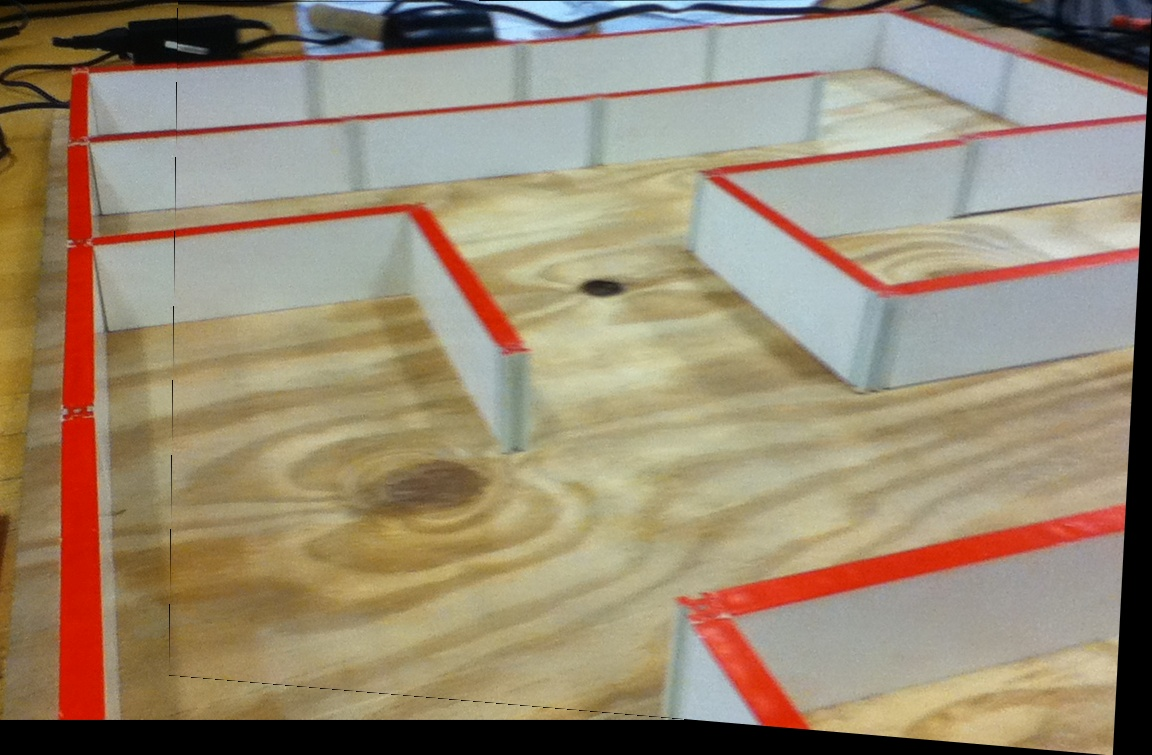
\includegraphics[width=0.8\linewidth]{../../src/imgs/one.jpg}
	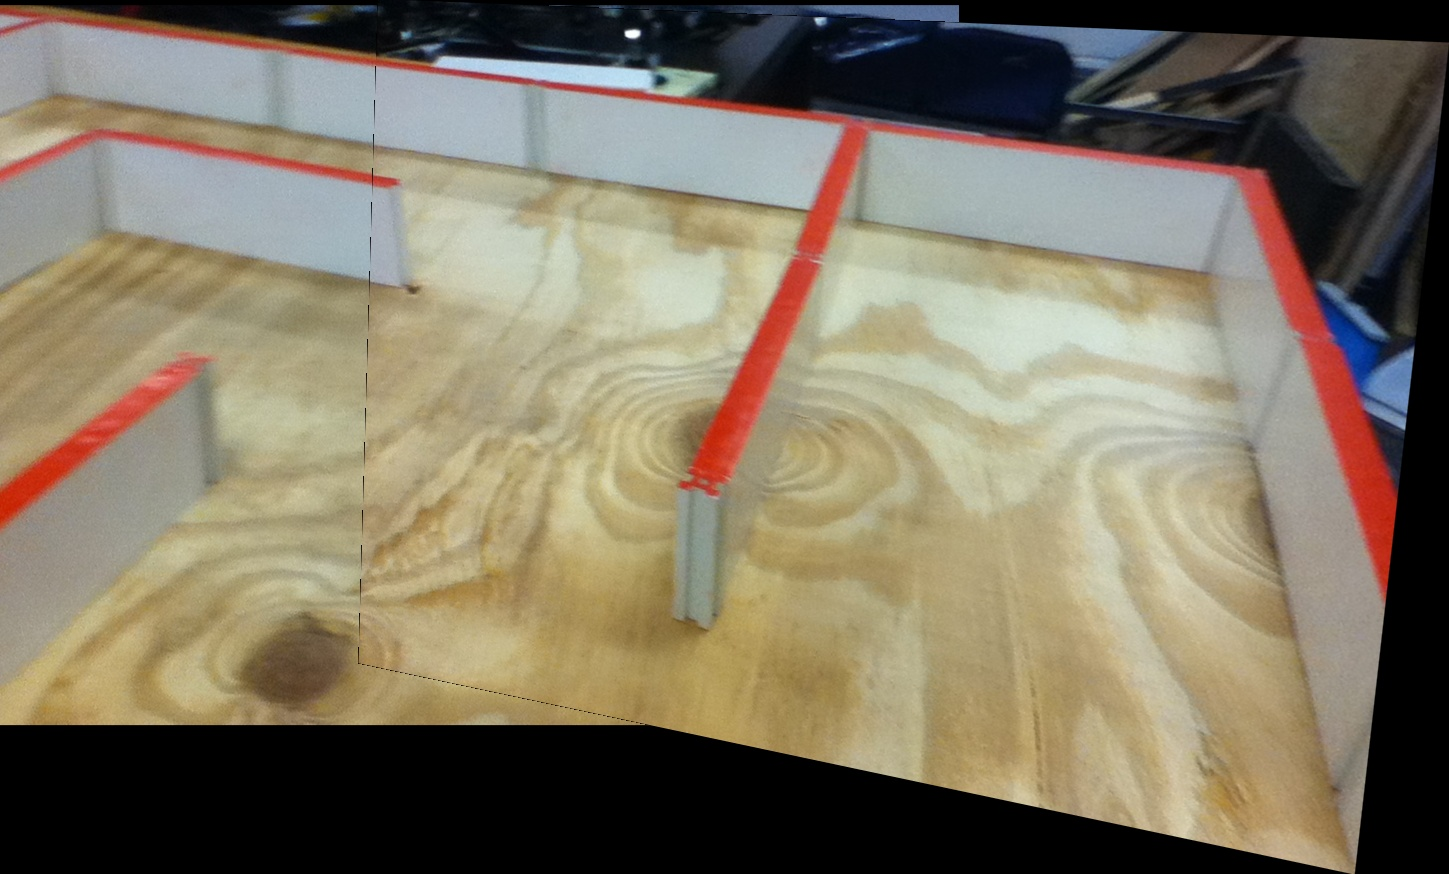
\includegraphics[width=0.8\linewidth]{../../src/imgs/three.jpg}
\end{center}
\caption{Example stitched maze images from the mouse's perspective.}
\label{fig:stitched}
\end{figure}

After obtaining a set of stitched images, we begin performing image transformations.  Because the end goal is to produce
an orthographic image of the maze from the point of view of an observer looking down from directly above the maze, we
use homographies to transform the stitched source images.  The high-level steps necessary for doing so are reproduced
below.
\\
\\
\textit{For each stitched image:}
\begin{enumerate}
	\item Find all lines in the image using the Hough line transform- these lines usually lie along, or near, maze
	walls.
	\item Since walls have finite thickness in space, the Hough transform will find multiple lines with similar slope
	and intercept for each wall.  Divide the lines into groups according to slope, and further subdivide by intercept.
	\item Obtain a single line for each wall by removing outliers in every cluster and then averaging slope and
	intercept.
	\item Compute all points in the image where the averaged Hough lines intersect.
	\item Treating the intersection points as polygon vertices, find all closed polygons in the image.
	\item Identify the polygon enclosing the smallest area, since this is likely to be the perspective view of a square
	in the maze.
	\item Compute the homographic transformation between the stitched image and a top-down view of the same scene by
	using the corners of the aforementioned polygon and the corners of a square centered in a $3000\times 3000$-pixel
	image as keypoints.  The large size of the target image is chosen so that the source image, after being transformed
	by the homography (which stretches some regions) does not experience boundary clipping.
	\item Crop the transformed image by finding the smallest rectangular region that bounds the image information (most
	of the pixels of this image will be zero, and the transformed, stitched image will occupy a small quadrangle near
	the center).
\end{enumerate}

In essence, this set of steps automatically finds the maze walls under perspective projection (as they appear in the
images from the mouse's point of view), and then attempts to transform each image using the prior knowledge that each
polygon enclosed by the maze walls is, in reality, a square, and would be seen as such from a top-down point of view.

In the final stage of the algorithm, all of the previously-stitched and transformed images, which now appear as pieces
of a top-down maze view, are stitched together, and the same linefinding technique as before is used to identify the
walls of the maze.  The output of the algorithm is a textual encoding of the locations of all maze walls, which can
directly be fed to a Micromouse to be solved and executed.  Therefore, after all transformed images have been obtained:

\begin{enumerate}
	\item Stitch all transformed images together to produce a single, top-down view of the maze.
	\item Perform the Hough line transform again to approximate the grid on which all maze unit cells lie.
	\item Center the lines generated by the Hough transform onto the walls of the maze by taking a window of pixels
	around each line and shifting the line towards regions with red pixels, which are likely to be maze walls.
	\item Find the intersection points of the grid in the image.
	\item Extract a digital representation of the wall locations. (HOW???)
\end{enumerate}

After the wall locations have been determined, the optimal maze-solving path can be determined using standard 
graph-theoretic methods, and the mouse can consequently solve the maze.

\section{Results}
\label{sec:results}

We implemented our algorithm using the Python language along with the OpenCV, NumPy, and matplotlib packages for
computer vision and image processing, and numerical computation, respectively.  We chose this platform over MATLAB and
C++ (which also has support for OpenCV) to reduce implementation time, in order to be able to devote more effort to
high-level algorithmic development.  Also, the flexibility of Python in comparison to MATLAB for performing 
"non-numerical" tasks such as file input and output and project management made it a natural choice.

\subsection{Output images}
\label{sub:output_images}

In this section, we present several images representative of the output of our algorithm at various stages of execution.


\section{Discussion}

Note that the images used for development and testing purposes (examples of which are shown in figure
~\ref{fig:stitched}) are of a $4\times 6$-cell maze, instead of the full-size $16\times 16$.  In order to capture images
with enough infor

\label{sec:discussion}
\subsection{Earlier Solution Attempts}
\label{sub:earlierattempts}

Our first attempt at a solution to this problem consisted of using trigonometric information to obtain an orthographic projection 

\subsection{Difficulties Encountered}
\label{sub:difficulties}
\begin{itemize}
	\item SIFT matching not working (trying to perform image stitching ourselves)
	\item Trying to manually retrieve an orthographic projection in 2 dimensions
	\item Finding a way to get the corners of the smallest square in a consistent order to use in the homography
	transformation
	\item Finding a good way to reduce the number of Hough lines down to a simple grid
\end{itemize}

\subsection{Future Work}
\label{sub:futurework}
\begin{itemize}
	\item Implement the software on a working Micromouse
	\item Learning how to use real camera data, which may not be as good as what we were able to achieve here
\end{itemize}

{\small
\bibliographystyle{ieee}
\bibliography{references}
}

\end{document}
